\documentclass[12pt,letterpaper]{article}

\usepackage{graphicx}
\usepackage[utf8]{inputenc}
\usepackage{mathtools}
\usepackage[margin=0.5in]{geometry}
\usepackage{booktabs}
\usepackage{tabu}
\usepackage{caption}
\usepackage[labelfont=bf, skip=5pt, font=small]{caption}
\usepackage{hyperref}
\usepackage{siunitx}
\usepackage{standalone}
\usepackage{import}
\usepackage{stanli}
\usepackage{tkz-euclide}
\usetikzlibrary{calc}
\usetikzlibrary{patterns,arrows.meta}
\usetikzlibrary{shadows}
\usetikzlibrary{external}

\hypersetup{
    colorlinks=true,
    linkcolor=blue,
    filecolor=magenta,      
    urlcolor=cyan,
    }
\usepackage[font=footnotesize,labelfont=bf]{caption}
\setlength{\parskip}{1em}
\setlength{\parindent}{0em}




\let\DeclareUSUnit\DeclareSIUnit
\let\US\SI
\DeclareUSUnit\inch{in}
\DeclareUSUnit\lbf{lbf}
\DeclareUSUnit\lb{lb}
\DeclareUSUnit\psi{psi}
\DeclareUSUnit\ksi{ksi}
\DeclareUSUnit\Msi{Msi}











\begin{document}
\section{Impact Duration}

In order to determine an impact duration appropriate for landing, a series of test where preformed to estimate the impact time. Using a drone which is similar in size and mass (960g) to the ContraHopper, dropped from various heights repeatedly, a very rough estimate on two different parameters can be achieved. Its important to note that this is by no means an thorough and definitive answer to this question. The model is vastly over simplifying a complex interaction, results should be used indicate a ballpark including the parking-lot answer. 

\begin{itemize}
    \itemsep -3pt {} 
     \item Estimated Impact Time
    \item Validity of rigid body inelastic impact model
\end{itemize}
The impact model is based on rigid body kinematics, and a inelastic collision.
\begin{gather}
\begin{aligned}
    &F_l = ma 
    \\
    &a = \frac{\Delta v}{\Delta t}
    \\
    &\Delta v = v_l = \sqrt{2gh}
    \\
    &\Delta t = \frac{\sqrt{2gh}}{a}
    \\
    &F_e = m\frac{\sqrt{2gh}}{\Delta t}
\end{aligned}
\end{gather}

\begin{description}
    \item $F_l$ = Landing Force
    \item $F_e$ = Estimated Landing Force
    \item $m$ = Mass of Vehicle 
    \item $a$ = Deceleration on impact  
    \item $\Delta t$ = Time of Impact
    \item $v_l$ = Landing Velocity
    \item $g$ = Acceleration of Gravity
    \item $h$ = Distance Vehicle Falls
\end{description}

Some of the concerns I have about the results of this test are in the accuracy of the accelerometer measurements as well as the sample rate. Each test was repeated as many times as my neighbors would allow. The IMU being used is a mpu6050, with the following settings:

\begin{description}
    \item Log Rate = 200hz
    \item Accelerometer Full scale Range = +-16g
    \item Accelerometer Calibration Method = Post-Logging Mean Offset
\end{description}

Additionally, I am dropping the drone from marking on a tape measure by eye, there is likely an error in the height measurement.

\pagebreak


\section{Results}


\begin{figure}[h!]
\centering
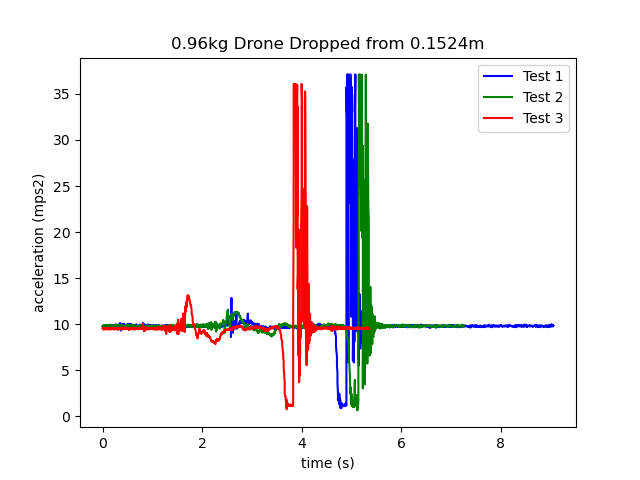
\includegraphics[width = 0.75\textwidth]{Impact_Fig/6in.png}
\end{figure}

\begin{figure}[h]
\centering
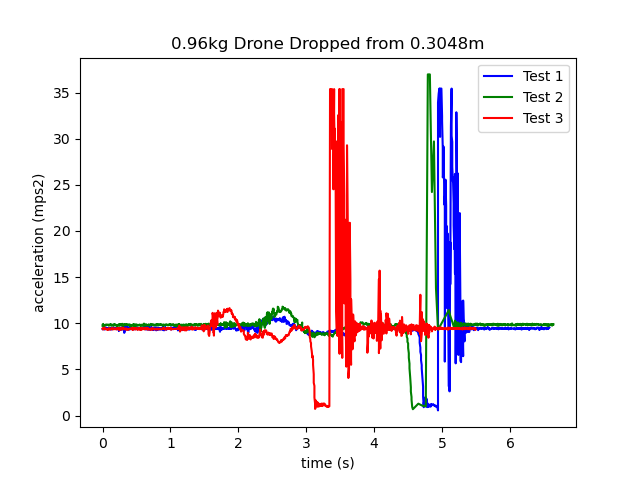
\includegraphics[width = 0.75\textwidth]{Impact_Fig/1ft.png}
\end{figure}

\begin{figure}[h]
\centering
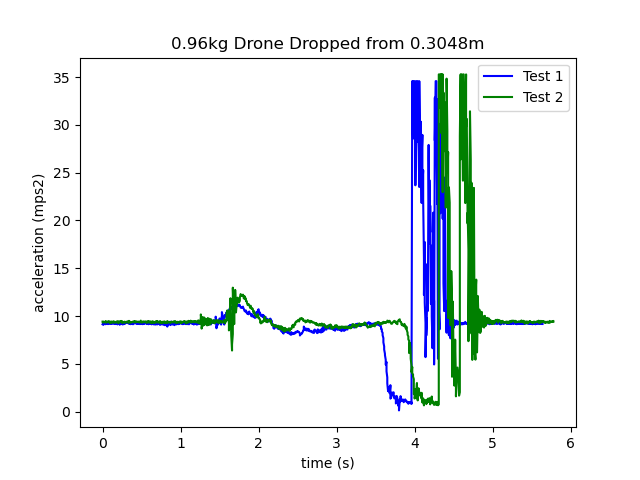
\includegraphics[width = 0.75\textwidth]{Impact_Fig/2ft.png}
\caption{0.6096m Accelerometer Data}
\end{figure}

\section{Notes}


Unfortunately, this shows data that with the current configuration I will be unable to measure impact time, or loads. This does indicate that I should expect at least 4gs, more than that is unkown.
\end{document}